\documentclass[border=10pt]{standalone}
\usepackage{tikz}
\usepackage{pgfplots}
\pgfplotsset{compat=1.8}

\begin{document}
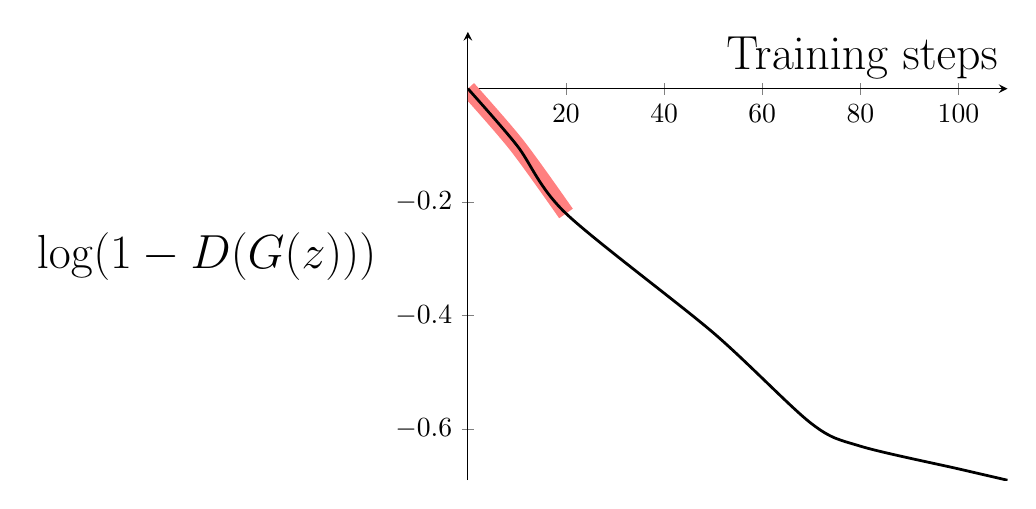
\begin{tikzpicture}
	\begin{axis}[
		xlabel={Training steps},
		axis lines=middle,
		ylabel near ticks,
		ylabel={$\log(1 - D(G(z)))$},
		ylabel style={rotate=-90, font=\LARGE},
		xlabel style={font=\LARGE},
		ymax=0.1
	]
	
		% shading
	\addplot[line width=6pt,color = red!50, domain = 0:0.2, smooth]
	coordinates {
	(0, 0)
(10,-0.1)
(20,-0.22)};
	
	% use TeX as calculator:
	\addplot [mark=none,domain=0:1, line width=1pt, smooth] coordinates {
		(0, 0)
		(10,-0.1)
		(20,-0.22)
		(50,-0.43)
		(70, -0.59)
		(80, -0.63)
		(100, -0.67)
		(110, -0.69)};

	\end{axis}

\end{tikzpicture}

\end{document}